\chapter{Parallelisierung}
\label{chp:para}

\section{Topologie}
\label{sec:topo}
Da das Programm nebenläufig sein sollte, mussten wir eine Topologie
erstellen, damit die Kommunikation zwischen den einzelnen Prozessen
festgelegt wird.

Zunächst wollten wir das Programm mehrmals unabhängig voneinander
laufen lassen, wobei zwischendurch immer wieder untereinander
kommuniziert wird, wie in Abbildung~\ref{fig:mult-pop} dargestellt.
Der Hauptprozess erhielt sporadisch die beste Rundreise eines
Prozesses und war in der Topologie nur für das Initialisieren und
Beantworten von Nachrichten des Benutzers zuständig.

\begin{SCfigure}
  \centering
  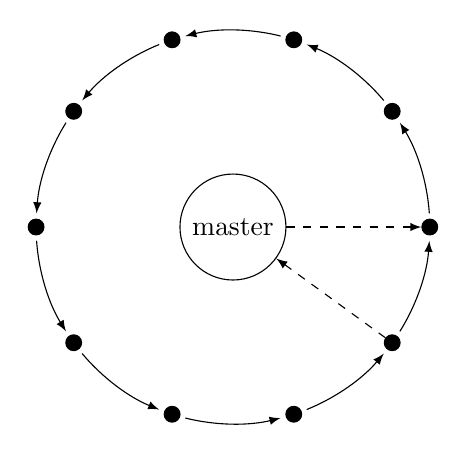
\begin{tikzpicture}
    [place/.style={circle,
      inner sep=0pt,minimum size=2mm}]
    %% from http://www.texample.net/tikz/examples/cycle/
    % Author : Jerome Tremblay
    \def \n {10}
    \def \radius {2.5cm}
    \def \margin {4} % margin in angles, depends on the radius

    \foreach \s in {1,...,\n}
    {
      \node[draw, circle, fill=black, place] (\s) at ({360/\n * (\s - 1)}:\radius) {};
      \draw[->, >=latex] ({360/\n * (\s - 1)+\margin}:\radius)
      arc ({360/\n * (\s - 1)+\margin}:{360/\n * (\s)-\margin}:\radius);
    }

    \node[draw, circle] (master) at (0:0) {master};
    \draw[->, >=latex, dashed] (master) -- (1);
    \draw[->, >=latex, dashed] (\n) -- (master);
  \end{tikzpicture}
  \caption[Mehrere Populationen]{\label{fig:mult-pop}Es werden mehrere
    Populationen erzeugt, die dem jeweils nächsten Prozess dann Teile
    aus der eigenen Population zusenden.

    Der Hauptprozess empfängt hier nur sporadisch neue Rundreisen und
    antwortet hauptsächlich auf Nachrichten von dem Benutzer.}
\end{SCfigure}

Dabei stießen wir auf mehrere Probleme.  Zum einen mussten wir selber
einen Garbage-collector implementieren, der sich um das Löschen von
Graphen kümmern sollte.  Da dies aber asynchron verlief, konnte es zu
„race conditions,“ bei denen ein Graph gelöscht wurde und danach ein
Prozess diesen in die eigene Population aufnehmen wollte, kommen.

Deshalb wurde der Aufbau so verändert, dass der Hauptprozess alle
Kindprozesse instruiert jeweils einen Offspring zu erzeugen und diesen
wieder zurückzuschicken (vgl. Abbildung~\ref{fig:topology-central}).
Da in diesem Fall aber die Population zentral verwaltet wurde, mussten
neue Rundreisen sequenziell in die neue Population einsortiert werden,
was der Nebenläufigkeit schadet.  Darüber hinaus konnte während dieses
Zeitraums der Status nicht abgefragt werden, da der Hauptprozess
während dem Erstellen der nächsten Generation blockierte.

\begin{SCfigure}
  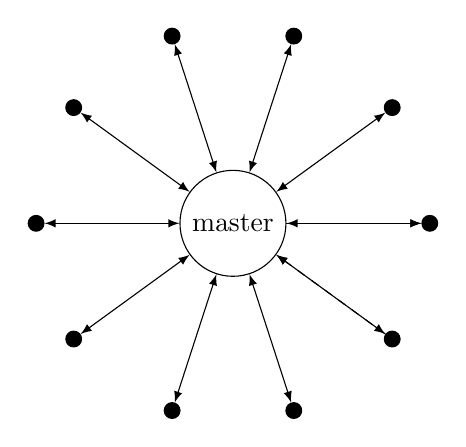
\begin{tikzpicture}
    [place/.style={circle,
      inner sep=0pt,minimum size=2mm}]
    \def \n {10}
    \def \radius {2.5cm}
    \def \margin {4} % margin in angles, depends on the radius

    \node[draw, circle] (master) at (0:0) {master};

    \foreach \s in {1,...,\n}
    {
      \node[draw, circle, fill=black, place] (\s) at ({360/\n * (\s - 1)}:\radius) {};
      \draw[<->, >=latex] (master) -- (\s);
    }

    \draw[->, >=latex, dashed] (master) -- (1);
    \draw[->, >=latex, dashed] (\n) -- (master);
  \end{tikzpicture}
  \caption[Verteilte Erzeugung von Offsprings]
  {\label{fig:topology-central} Die Kindprozesse erzeugen einzelne
    Rundreisen und schicken diese an den „master“ zurück.  Dieser muss
    die Rundreisen dann in die eigene Population einsortieren.}
\end{SCfigure}

\section{ETS-Tabellen im Netzwerk}
\label{sec:ets}

%% ets tables
Das normale Limit von Datenbanktabellen liegt bei
1400 Tabellen pro Node.\footnote{\url{http://erlang.org/doc/man/ets.html}} \hskip2pt Da
ein Graph aus jeweils drei Tabellen besteht, können wir unser Programm
nicht beliebig skalieren, da sonst das Limit auf einer Node erreicht
wird.  Erhöht man die Grenze, so degradiert die Geschwindigkeit der
virutellen Maschine, wenn zu viele Tabellen vorhanden sind.  Darüber
hinaus werden diese nicht von der Garbage-collection gelöscht sondern
müssen manuell freigegeben werden.  Eine Tabelle hat allerdings immer
einen Besitzer und nur dieser hat das Recht den Speicher einer Tabelle
aufzulösen.  Benutzen nun also mehrere Prozesse die selben Tabelle,
muss der Besitz auf einen anderen Prozess übertragen werden, bis nur
noch ein Prozess diese Tabelle benutzt.  Dieser kann dann die Tabelle
löschen.  Dass ein Graph so behandelt werden muss, ist nicht
offensichtlich und benötigt Rechenzeit, die nicht für den
evolutionären Algorithmus selbst verwendet werden kann.
